\chapter{从AI到最佳设计} % Introduction chapter suppressed from the table of contents


``我们现在推行AIGC，服务端不需要UI交互设计的用AI自动产出代码，你建议的结对编程、TDD等是否还适用？''\\
这两年AI确实很火，是报纸、杂志的热门话题。例如，HBR杂志从2024年9月至2025年二月份3期，里面有接近一半文章都与AI有关。朋友圈晚饭或在飞机场候机厅我都提过以下对话：\\
``未来人类的工作估计全都会被人工智能取代！''\\
``以前以为有些专业，例如医生，会比较放心，难以被AI替代，但听说好像连手术也可以由机器人来做了。''\\
越来越多开发团队使用AI，希望提高效率。如何能有效地利用AI？应如何适应这新技术发展？
详细讨论这些之前，先分享两个故事：\\

\hypertarget{ux4e24ux4e2aux6545ux4e8b}{%
\subsection{两个故事}\label{ux4e24ux4e2aux6545ux4e8b}}

某欧洲城市巴士公司为了提升效率管理层引入了奖金计划：按计划不延误，给司机的奖金越高。\\
因为巴士按区收费，售票员也要查看下车乘客有没有正确按规定买票，公司会随机随机派人抽查，如发现售票员违规（包括售票与查票）会扣奖金。因为收入提升，司机或和售票员都喜欢新的奖金制度。售票员在巴士后方有固定位置，指示司机是否可以开车离站。但当交通繁忙时，因乘客太多，太忙，售票员可能来不及回到车尾位置指示开车，这类延误会影响到司机的奖金收入。售票员大部分是少数民族新移民，司机大多是来自传统蓝领阶层，经常发生纠纷，有时候甚至会双方动手打人。请问有什么解决方案建议？\\
改善奖金制度？例如：平均分配奖金？请双方代表坐下来协商？一起讨论解决方案？

最终解决方案：\\
因为发现主要的繁忙车站数量比巴士数量少，所以安排售票员守在车站，在巴士到站前预先售票，售票员也可以在车站查看下车的乘客是否买了正确的车票；也可以在车站指示司机是否可以开车。非繁忙时间售票员可以正常回到巴士里工作。

\begin{description}
\item[]
\begin{description}
\tightlist
\item[]
-\/-\/-+++-\/-\/-
\end{description}
\end{description}

美国一家历史悠久的彩色印刷公司，主要为高端的杂志和出版社印刷彩色照片或者油油画等。公司在美国俄亥俄州有8条生产线，虽然销售还是很理想，但管理生产的副总裁VP要解决一个头疼的问题------过去5年生产线的生产率逐年下降，甚至已经开始没有利润。通过检查设备、机器是否老化、设备缺乏维修等，发现这些都不是原因。最后发现主因是虽然增加了大量新产品，生产量却很少，而每一轮生产之间的准备时间却要增加很多，便请顾问看看如何优化生产的时间安排，希望能尽量减少准备时间。\\
顾问先用电脑对生产进行模拟，发现如果改善策划，确实能提高生产率。但顾问同时也发现产品线中绝大部分的利润来自8\%的产品，它们构成所有生产的9成。另外很多``老''产品，销售量很小，基本没有利润。发现这情况后，顾问跟生产副总裁提建议，但被拒绝------``卖什么产品，不是我们管生产的范围。''就请他问管市场部的副总裁，副总裁虽然没有拒绝，但担心影响客户满意度也不愿意取消老产品。因为这家老公司承诺客户永远不会停掉某一条已经提供过的产品线。\\
顾问还是觉得问题的核心不在调整生产，建议修正销售人员的分成安排：基本薪水不变，但他们的分成会按销售是否有利润挂钩。如果他们多卖一些有利润的产品，他们的收入就会提高。但如果他们多卖一些没利润的产品，对他们的收入没有帮助。人事部对这个建议很感兴趣，愿意找美国某区域做试点，试点发现有65\%没有利润的产品在整个试点区内就没有销售，但有利润的产品就提升了18\%，销售人员的收入加倍，然后公司的总收入也上升了一倍。

\begin{description}
\item[]
\begin{description}
\tightlist
\item[]
-\/-\/-+++-\/-\/-
\end{description}
\end{description}

以上两个故事的经验教训：

\begin{itemize}
\tightlist
\item
  改善系统的某部分不能改善整个系统
\item
  解决问题应从各种视角看，如果仅仅某个专业来分析，难以找出整个系统的最佳方案
\end{itemize}

在软件开发公司也有类似例子，比如专门给医院做系统的公司发现80\%开发出来的功能没有用上，浪费资源。改善开发流程并非问题的核心，而应针对怎么去挑选并拒绝没有价值的需求，公司组织里面的功能互相依赖，好比我们人体器官相互依赖，不能单靠优化某一部分改善整个系统。

\hypertarget{ux5411ux7164ux77ffux5de5ux4ebaux5b66ux4e60}{%
\subsection{向煤矿工人学习}\label{ux5411ux7164ux77ffux5de5ux4ebaux5b66ux4e60}}

战后50年代的英国煤矿，在机器化前，煤矿工人都是小组手工运作，伙伴互相帮助，后面利用机械化大规模采煤，类似工业生产的生产线一样，本以为设计好整个系统，配上工人，就能大大提升效率。但发现并非如此，机械生产开始时，按技能要求分工，如钻洞、切割、修建隧道、挖煤、清理等，每人负责一小块固定的工作，轮班
（详见附件的图2），发现工人常常生病，出勤率也不理想。必须安排后备人员，因某些岗位缺人会影响整个过程。\\
因煤矿是天然产生，煤层（分布、厚度等）会按地形变化。例如，如果最后挖煤的人发现前面负责挖洞工人没做好，挖煤便很困难。机器化之前都是团队制，互相依赖，互相帮忙解决问题。但现在工作细分后，当挖煤的工人遇到困难时便求助无门，很无奈，导致大量缺勤、生病。\\
针对这不足，有些公司采用多功能团队制，让团队可以灵活按需要转换工种，不是只做某一块工作，像机械化前互相合作，发现效果很好，生产力从以前的78\%提升到95\%；旷工率从20\%
降到8.2\%。（详见附件）\\
从以上研究发现，不能仅仅靠科技设计生产线，也必须考虑人的因素，E.Trist
、F.Emery 等学者提出社会技术系统 socio-technical systems (STS)
的概念，工人不是生产机械的延续。

\framebox{%
\begin{minipage}[t]{0.97\columnwidth}\raggedright
1936年的经典黑白电影《摩登时代》(Modern
Times)，卓别林演电影中的工厂工人，每天不断地做一项工作：拧螺丝钉。最终顶不住烦躁的工作，发疯了，借此讽刺工业生产线生产的问题。
\strut
\end{minipage}}

软件开发也一样。\\
前面章节提到有些公司从需求到测试每个环节分工明确，某些岗位只做需求，某些岗位只做设计，误以为每个环节做好，总体的效果一定会好，忽略了活动间相互依赖。例如需求写得模糊会导致开发和测试出现缺陷和返工。这些都要等到测试和验收时才发现，但正因为每个工种独立，做开发或测试的很无奈，因为心里都知道，问题是出自需求，但她控制不了。所以敏捷开发强调要小团队各人互补。\\
例如：测试报告：\\
因为测试只能从他的视角看到有多少是系统测试找出的缺陷做分析，没有考虑其他过程，如评审，需求等，不清楚缺陷的真正源头，报告对减少后面缺陷与返工没有帮助。但是如果所有团队成员，包括需求、开发一起分析缺陷的排除率，就可以更全面的看到问题了。\\
``我们确实有类似以上的问题，但如果要改善整个系统有什么好办法？''\\
``请问你现在电话的一些功能，例如：

\begin{itemize}
\tightlist
\item
  按键音频电话、呼叫等待、呼叫转移、语音邮件、来电显示、电话会议、免提电话、快速拨号
\item
  touch tone phone , call waiting, call forwarding, voice mail, call ID,
  conference call, speaker phone, speed dial in memory\\
\end{itemize}

是什么时候发明？''\\
以上功能都是1951年在美国贝尔实验室创造出来的。例如，按键音频电话机之前的电话都是拨号盘式。现在可能只能在某些古典酒店大堂看到，而且都是假的。

\hypertarget{ux5e74ux8d1dux5c14ux5b9eux9a8cux5ba4ux7684ux4f1aux8baeux5ba4}{%
\subsection{1951年，贝尔实验室的会议室}\label{ux5e74ux8d1dux5c14ux5b9eux9a8cux5ba4ux7684ux4f1aux8baeux5ba4}}

``全美国的电话系统昨晚被切底破坏，一无所有了。''召集紧急会议的副总裁很严肃，跟所有部门经理说。\\
``你们各位最好相信我刚才这番话，如果到了中午你们还不相信的话，我就辞退你。''\\
所有经理都莫名其妙，想``今天早上我才打过电话，这位副总裁出了什么问题？''\\
过了一会，副总裁面露笑容，原来他是跟大家开玩笑。\\
然后他解释说，``很多美国人都相信我们实验室是全美国最优秀的研发实验室。请问贝尔实验室对电话系统的最大贡献是什么？''\\
``转盘式 (dial) 电话''\\
%\href{文件:Rotary_dial_phone_Screenshot_2025-02-11_091618.jpg}{200px}


\includegraphics[width=10cm]{Rotary_dial_phone_Screenshot_2025-02-11_091618.jpg}

``同轴电缆 (coaxial cable)，经过大西洋连接美国和英国''\\
``但这些伟大发明都在1900年前，都是在座的所有人出生之前
，你们都只是对电话系统做了些改善，没有什么更大的贡献。\\
要做出有突破的优秀发明，先有以下2假设：

\begin{enumerate}
\tightlist
\item
  假定现在的系统已经被彻底破坏，从零开始想象希望电话系统有什么功能和好处？而且只是针对现在，不是五年或者十年以后。
\item
  不要顾虑有任何困难，先从客户的角度提出。\\
\end{enumerate}

但还要考虑2个限制条件：

\begin{itemize}
\tightlist
\item
  技术方面是否可行，我们不希望只是一个科幻小说的场景
\item
  在现在环境可操作，因为我们不可能改变环境，包括所有的法律、规章制度等\\
\end{itemize}

我们这么多人不可能一起设计，先把你们分成6个小组，包括：

\begin{itemize}
\tightlist
\item
  城市内的短途通信
\item
  城市间的长途通信
\item
  交换机
\item
  电话机等\\
\end{itemize}

现在大家开始分组讨论。''\\
上面提过(包括按键式电话)
的多种现代电话功能，都源自在当天分组互动工作坊里电话机小组的头脑风暴讨论。（工作坊时间有限，组员先从用户的角度，会遇到什么困难，想象有了新功能想法后，还是要与工程部交流，探索可行性。）\\
以上是Dr Ackoff
教授1951年的亲身经历，这次经历促进他在2006年出版《最佳设计》(Idealized
Design,详见参考)。他提倡要做好设计应：

\begin{itemize}
\tightlist
\item
  大家天马行空没有任何顾虑和限制，不考虑现在系统
\item
  不去分析现在系统的不足
\item
  工作坊形式交流与头脑风暴：没有公司岗位级别的区分，每个人都可以畅所欲言
\item
  因为这些经理都有参与开头的讨论，后面他们才会支持并投资源实现这些新发明\\
\end{itemize}

这最佳设计思路也适用于改善过程。我会经常利用在这类工作坊来帮助企业做过程改进，强调4点工作坊原则：\\
* 包括整个系统 Whole system in the room.

\begin{itemize}
\tightlist
\item
  从全局``全象''策划本身行动 Global``whole elephant "context for local
  action.
\item
  关注未来和共同点，而不是问题和冲突 Focus on future and common
  ground-not problems and conflicts.
\item
  自我管理，对行动负责 Self-management and responsibility for action.\\
\end{itemize}

很类似《最佳设计》里提倡重点，因背后都是基于STS学者研究发现的原理。

\hypertarget{ux7ecfux9a8cux5206ux4eab}{%
\subsubsection{经验分享}\label{ux7ecfux9a8cux5206ux4eab}}

必须找到了合适的利益相关者参与，必须整个系统的代表在一起，才能包含各种视角，例如，发现原来开发或产品经理是不理解现场实施人员面对的问题，测试人员也不知道开发人员面临的问题等。但当大家都聚在一起的时候，就可以交流、讨论如何改善整个系统。\\
主要部门负责人都要在，如果他们不在的话，所有新的思路会因为没有获得资源和支持，都很难推进。反过来如果相关人都有参与讨论的话，他们后面就有动力参与推行，因为觉得这是自己有出主意的东西。\\
也打破了公司里面的高低层的关系，每个人都可以自由发言，提意见。\\
如果刚才贝尔实验室的场景只靠高层副总裁定个年度计划，设定目标给一层一层去做创新，你估计会在短期内发生这么多新的创新变化吗？\\
不可能。个人的想象力有限，当然贝尔里面的人员每个都是行业精英，所以更容易在适合的环境，从整个系统看问题，做出突破。

\hypertarget{ux5f00ux53d1ux56e2ux961fux5982ux4f55ux5e94ux5bf9aiux5927ux8d8bux52bf}{%
\subsection{开发团队如何应对AI大趋势}\label{ux5f00ux53d1ux56e2ux961fux5982ux4f55ux5e94ux5bf9aiux5927ux8d8bux52bf}}

``AI实在太厉害了。AI围棋，初级，它让我6子，我还是赢不了。我以前一致认为电脑下象棋打败人类可信，但围棋太复杂了，一直不信电脑能学好这玩意。''我老同学聚餐时说，他从初中已经懂围棋，有超过40年下棋经验。

%\href{文件:围棋1.jpg}{300px}


\includegraphics[width=10cm]{围棋1.jpg}

越来越多人问人工智能帮公司提升生产率吗？我不懂人工智能，用手机下载了POE做一些查询，会导出一个很好看的报告，后面我再去细看的时候，发现里面有的信息是错误的。\\
例如，2025年2月初问：``Eric Trist Biography''

%\href{文件:Et.jpg}{300px}

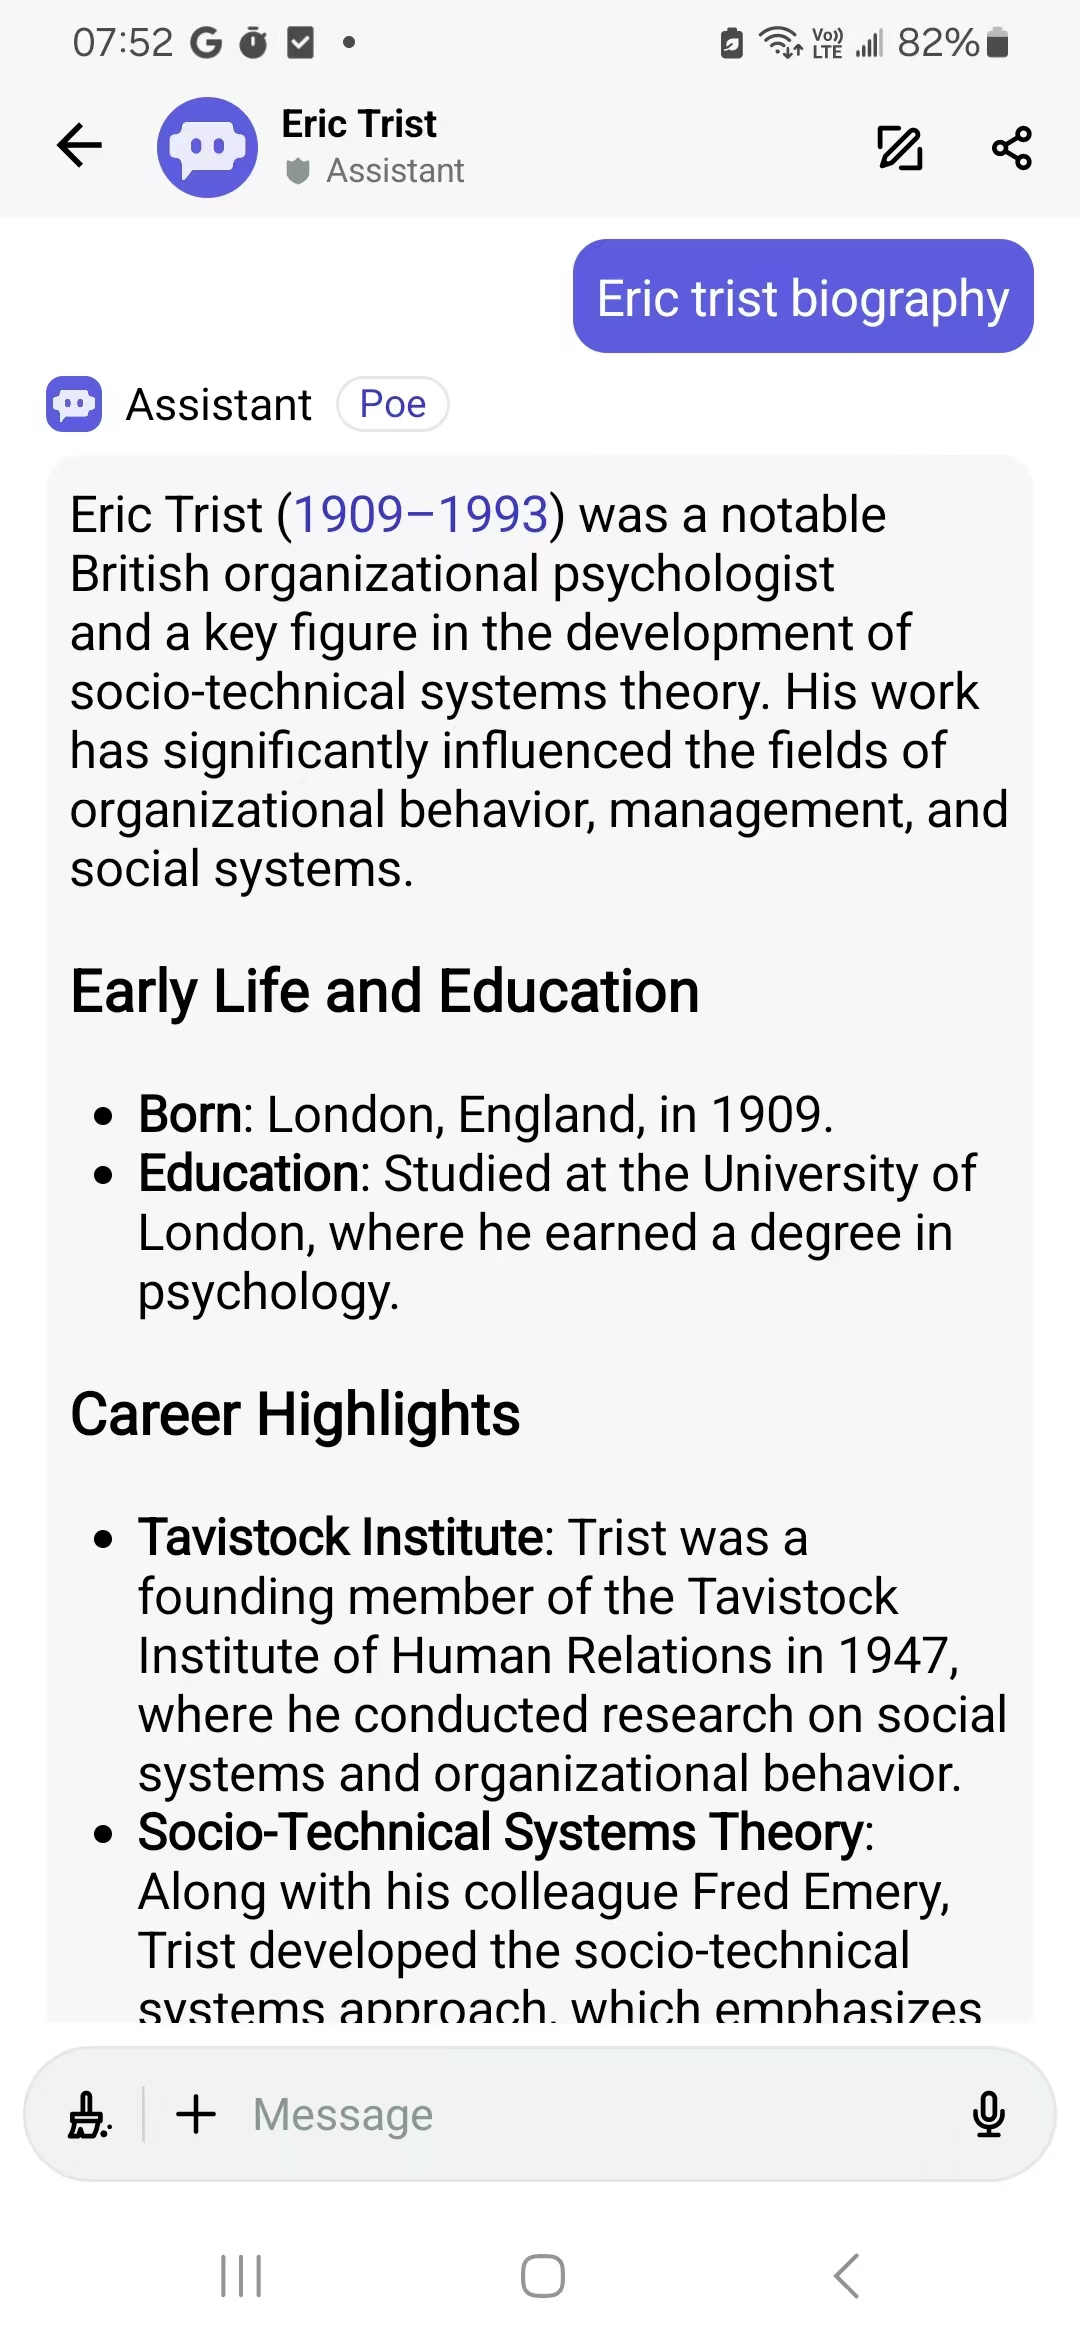
\includegraphics[width=10cm]{Et.jpg}

虽然格式包装都很专业，但内容有误：第一天：发现去世年份时2019年是错误的。第二天；同样再询问，（1909-1993）
是正确，但出生地点不是伦敦，他是剑桥大学毕业，非伦敦大学。
与能网上免费搜索到，如维基百科或Britannica出的内容相差甚远。\\
AI也可以自动生成PPT报告，并配上声音读出来。一些超过二十分钟的PPT，我通常看不到两分钟就离开了，因为太样板化，没有人气，就和打电话给人工智能客服一样，你会尽量想找个真人来跟你对话。\\
对比18分钟的TED讲话，讲者可能会先跟你开个玩笑或者挑某一件事引起你的兴趣，然后中间也会有停顿，有声调的高低，最重要会和现场的人有各种交流沟通，眼神、面容等，这些都是机器暂时无法替代的。也正是这些元素来吸引你，继续听完他的18分钟讲话。\\
以上实验暴露了AI的不足，因为它是靠大量搜索同类的文章信息，提供``最佳''答案，但中间可能缺乏检测过程，产生错漏，但客户（人类）可能误以为电脑出来的都是正确。所以虽然AI能很有效解决有明确规律的问题，如围棋，但难以取代人的思考与交流。而且与AI交流如进入了虚拟世界，难分真假。\\
所以有些研究发现程序员虽然用了AI自动生成代码，虽然代码多了，好像生产率提高了，但是缺陷数量也增加了。2024年的研究，分析了使用ChatGPT自动生成JAVA/Python程序，共四千个程序：发现40\%-89\%产出``正确''代码，看语言、难易度、是否有类似``老''程序供参考等因素。用静态扫描``正确''代码，发现各种代码异味（
详见附件）。\\
很多时候是初级的人员没经验，误以为自动生成的代码都是正确的，没去校验，就会出现问题。\\
所以大家不用担心AI会取代开发人员工作，因
AI只是有很大潜能的工具，类似80年代
IDE能提高开发效率，但无法超越人类，而且要小心使用。
因为AI自动出来的代码有不少缺陷，更需要我们前面提到的单元自动化测试，更需要团员间的评审，结对编程等确保代码的质量与可读性。更需要有环境让团队成员一起不断学习、不断交流、一起进步。最终人才最重要。（2023年，有家出名北京软件产品公司，我建议他们要有自动化单元测试，但开发主管说我的代码都是剂枪人自动生成，无法做到。所以他们内部集成、系统测试时，有些产品会以4位数的缺陷发现。）\\
所以丰田汽车的大野先生在五十年代引进机器人自动化的时候也特别小心，他不会以为买了机器人就能提升公司的生产率，必须要工程师想好怎么利用机器人辅助工作，确实能提高质量和效率才会批准购买。
我们也应该向大野先生学习，不要误以为用了AI就能提高效率，更需要看怎么可以辅助编码人员、开发人员、测试人员做好他们的工作。\\
如有固定规矩，偏重复性的工作，机器和AI能发挥作用
（如下棋、酒店送外卖到房间）；但要有创新的工作最终还是靠人。不要轻信短期未来人类会被人工智能取代，没有工作。\\
要做最佳设计还应参照1951年已经有公司成功使用的方法和原则。\\
AI只是一类新科技工具，每个人要更好学习提升才可以跟得上市场的竞争的最佳对策。\\
所以HBR2024年9月份一篇文章提到公司不应误以为AI是可以帮公司创造独特的竞争能力，原因是你可以用AI，你的竞争对手也可以很容易复制。（详见参考）

\hypertarget{ux603bux7ed3}{%
\subsection{总结}\label{ux603bux7ed3}}

虽然本部分分章节讨论需求、设计、编码、集成、评审、测试各过程的最佳实践，但若想改进应先设定总体目标，用多种视角看整个系统，再定各过程如何配合，好比建筑师按你的新花园别墅要求（如2层4房2厅，预算在一千万内）一样，必先做总体别墅设计，而不是先分别房间、客厅。

\hypertarget{ux9644ux4ef6}{%
\section{附件}\label{ux9644ux4ef6}}

\hypertarget{ux82f1ux56fdux7164ux77ffux751fux4ea7ux95eeux9898ux7684ux7814ux7a76}{%
\subsection{英国煤矿生产问题的研究}\label{ux82f1ux56fdux7164ux77ffux751fux4ea7ux95eeux9898ux7684ux7814ux7a76}}

在机械化之前，英国采煤是以小组作坊式工作,通常是两人一组，再加上一位做清理的助手。小组会直接跟矿场合作，专门负责某一块煤矿，小组以互补的形式做各种工作，自己管自己，独立性很高。因为采矿工作非常危险，所以选择伙伴很重要，都希望有稳定的伙伴关系，不会轻易换人。当某工人受伤或者去世，他的伙伴都会尽力帮助他的家人。这种小组作坊式工作方式后来被机械化生产线模式取代，但机械化生产却引起很多新问题。\\
先了解一下长壁（Longwall）开采法是怎么利用机械化大规模开采煤矿。\\
英国的煤层一般不深，最多可能1米左右，上面覆盖着泥土。用长壁机械化采煤方式就可以大面积采煤。

图1：\\
%\href{文件:煤矿图2.jpg}{500px}

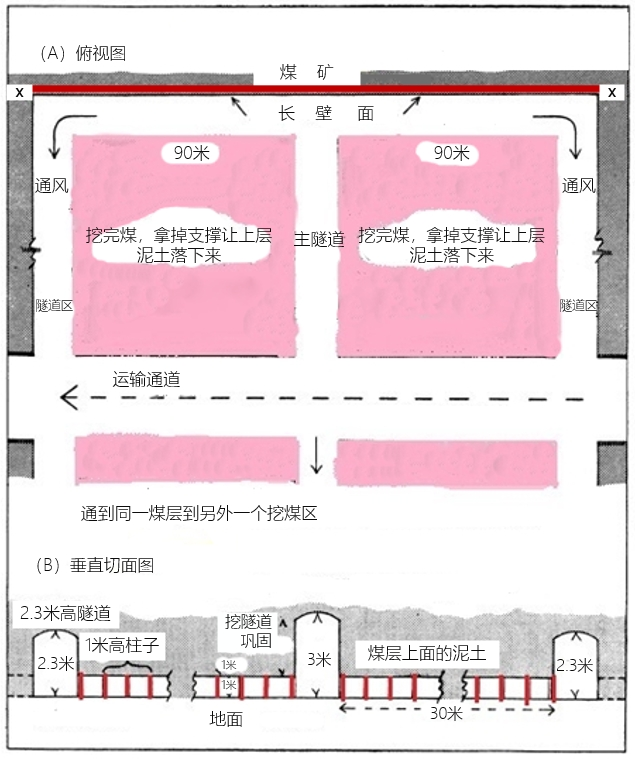
\includegraphics[width=10cm]{煤矿图2.jpg}

（上图A部分是煤矿俯视图，B部分是俯视图中长璧面从左面X 到右面X
直线的切面图，能看到是左、中、右3条隧道）

共180米宽的长壁是为了大面积采煤，（看上图）为了通风和运输，会有3条隧道，之间距离90米，中间隧道是比较高，大概有3米(9英尺)，左右隧道比较矮，大概2.3米(7英尺)高。这些隧道都是固定，让人或机械可以在中间通过。看上面平面图，左右2块90米宽的方形面积都是已经采完煤的泥土。从下面的切面图（B）
可以看到中间的和两边两个隧道。每个采煤的煤层，只有1米高。也可以看见1米高的柱子，柱子是用来顶住上面的泥土，防止泥土在煤挖空以后塌下来。

长壁（Longwall）如何操作：\\
沿长壁面X到X180米的直线有两条平行的过道，都是1米宽。贴着煤矿哪条一条只有1米高的通道，是让采煤工人爬过去工作。旁边有一条传输带运作的通道，也是一米宽，一米高。每一米都会有柱子顶住上面的泥土。当长壁180米的煤挖完后，会继续同样往煤矿开2条通道，拆掉原先的柱子，搬到新建2条通道使用。原先2条通道的上层泥土会塌下来。你可以想象挖煤工人沿着一米宽一米高的通道挖煤，放到旁边的运输带，工作环境多么恶劣。

工程师设计了7个工种，请参照下面的轮班表。每循环会包括3个轮班：

\begin{itemize}
\tightlist
\item
  第1个轮班主要是做转动和切割和清理，比如让那些切割的煤有空位落下来，让后面那些采煤工人容易可以采到煤。通常第一个轮班都是下午班或者晚班。
\item
  第2个轮班就是巩固隧道和安装传输带，通常是下午班或者晚班，这2个班总共就会大概有20个工人。细分到不同的工种，比如有2位只钻洞、2位只切割、8位专门管理通风隧道的巩固工作，分工很细。
\item
  第3个轮班主要有20位采煤工人操作。第3个轮班只有早上班和下午班，所以他们需要依赖前期技术人员做好准备工作，然后自己按大概9米的范围去采煤。收入是按采煤量计算，比如20位采煤人每人负责9米，加起来刚好等于整个长壁的180米。
\end{itemize}

分工设计很科学，如果都按正常操作，每次循环可以采到200吨煤。\\
图2： 工人分工和轮班\\
%\href{文件:长壁.jpg}{500px}

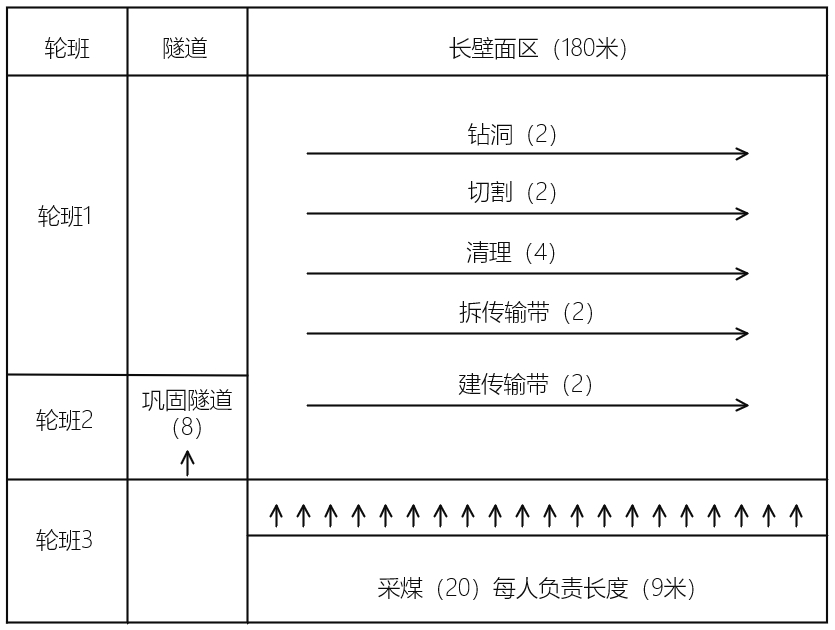
\includegraphics[width=10cm]{长壁.jpg}

但是你估计，这种机械化的大规模连续采煤操作会有什么问题？生产力效果怎么样？\\
以上的工作关系很密切，例如：

\begin{itemize}
\tightlist
\item
  如果洞钻得不够深，采煤工便采不到煤。
\item
  如果切割没做好会导致采煤工可采空间不足，影响产量。
\item
  如传输带没有安装好，不成直线就导致后面的传输停顿，采煤工无法操作。
\end{itemize}

各种状况都可能发生，加上煤矿是天然的，本身就有很多变数：例如地层有断层，或者地下天然气等。各种人为因素或天然因素都影响采煤工能否正常采煤。加上采煤的工作环境很恶劣，导致旷工问题很严重。例如某采煤工因前面2个轮班工作没做好，导致煤太硬，采不了，就需要用机器、工具去采，很辛苦，效果也不好，导致他工作2天就放一天假，然后也不补班。有些轮班因为人手不够，剩下的采矿工人就需要在地下多做两三个小时，才可以把整个长壁做完。最后当有些轮班时，采矿人数确实太少了，其他人也撂担子，导致无法正常开工。\\
因为采用机械化大规模采煤的各种问题，有些矿场开始引入自主团队组织架构，取代原本的轮班分工（下面称为传统分工）。\\
表1是两个不同的组织架构，技术都一样，也是在同一个环境。左面用原本长壁的方式设计工作分工，右面的加上自主团队负责制分工。左面矿工只需要做一项简单工作，比如采煤，与其他工人没有任何关系（在前面已详细举例说明）。右面就需要组员合作，协调应对采矿的各种特殊情况。\\
从这个例子看到同样一个采煤技术，可以有不同的组织架构支撑，效果完全不一样。所以团队组织架构必须与技术部分相配合，不能单独设计工人工作。

\textbf{表1:}\\
%Screenshotfrom2025-02-1720-41-57.png

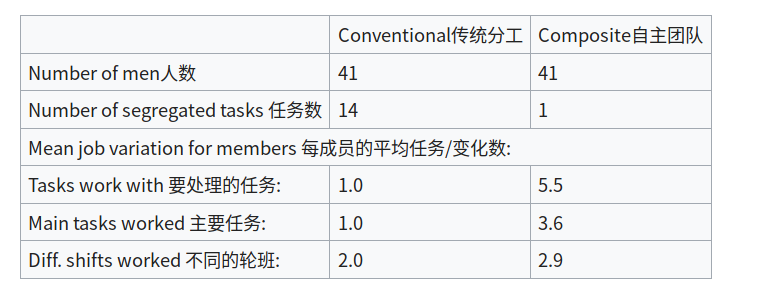
\includegraphics[width=10cm]{Screenshotfrom2025-02-1720-41-57.png}

从下面表2可以看到右面的组织架构更灵活，生产率比传统的单一工作设计高。右面的自主团队架构更能适应变化万千的采矿、采煤环境。采煤的步骤安排，也必须按照按环境的不同来应对。但如果是左面的硬性单一分工安排，缺乏这种灵活性（除非是专业性强的技术工种，必须把工作细分,每个人做某一件事)。但在采煤机械化、批量生产这种技术没有这个限制，所以采煤工人经过一些学习可以兼任其他工作。

\textbf{表2:}\\


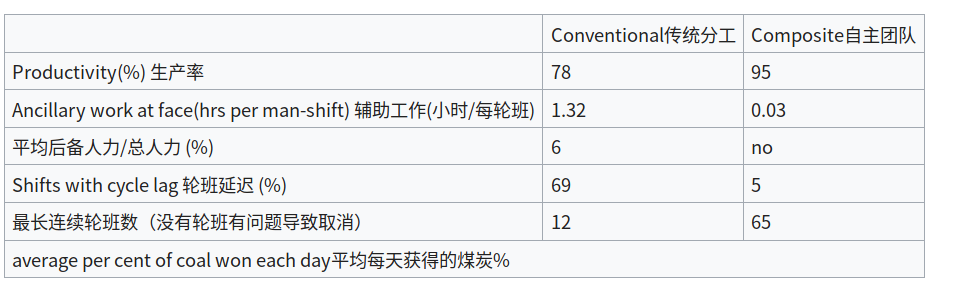
\includegraphics[width=10cm]{Screenshotfrom2025-02-1720-43-11.png}

团队组织架构除了让工人更好做好采矿工作以外，也可以更好满足工人的个人心理需要，包括互相支持，有团队合作的概念。但是如果按左面传统的工业化分工，就缺乏合作。导致很多采煤工只能单打独斗，孤立无援，导致心理压力很大。这个也可以从表3的缺勤率看得出来，会更容易无缘无故请假等，背后主因是分工设计导致工人心理压力太大，承受不了。团队互相协助的环境可以减轻这方面的压力。

\textbf{表3:}\\

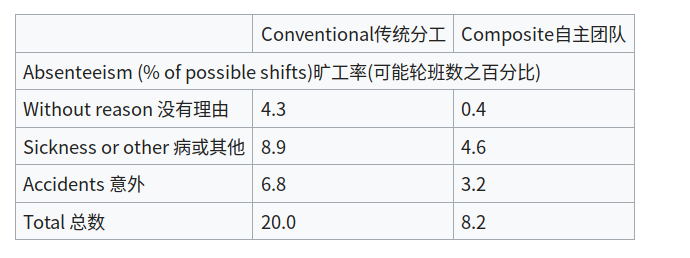
\includegraphics[width=10cm]{Screenshotfrom2025-02-1720-43-42.png}

\hypertarget{chatgpt-ux81eaux52a8ux751fux6210ux4ee3ux7801ux8d28ux91cfux7814ux7a76ux7ed3ux679cux91cdux70b9}{%
\subsection{ChatGPT
自动生成代码质量研究结果重点}\label{chatgpt-ux81eaux52a8ux751fux6210ux4ee3ux7801ux8d28ux91cfux7814ux7a76ux7ed3ux679cux91cdux70b9}}

2024年发文的研究分析了4066个ChatGPT
自动生成的JAVA/Python程序，发现2756个正确（约占68\%），1082个结果不正确，177个编译出错。

\begin{itemize}
\tightlist
\item
  成功出正确结果\%与程序难易度相关，容易的程序成功率最高，难的成功率最低，JAVA
  与 Python 一样
\item
  Mann-Whitney U 测试JAVA与Python间的差异是否显著P-value都大于0.05
  ,差异不显著（详见下表）
\end{itemize}

表1：LeetCode的通过率准确率



\resizebox{\linewidth}{!}{

\renewcommand{\arraystretch}{1.5}

\begin{tabular}{|c|c|c|c|c|c|}
\hline
Pass@1 & 低 Easy & 中 Medium & 高 Hard & 总 Overall\\
\hline
Python & 0.890 & 0.674 & 0.400 & 0.664\\
\hline
Java & 0.860 & 0.710 & 0.468 & 0.691\\
\hline
P-value & 0.346 & 0.654 & 0.535 & 0.471\\
\hline
\end{tabular}

}






\begin{itemize}
\tightlist
\item
  也取决于这程序是否新出现，越新越容易出错（因ChatGPT难以从网上找到参考例子）：
\item
  下图最右是2023年1月后，最左是2021年7至12月
\item
  难度越高，新旧间的差异越大\\
\end{itemize}

%\href{文件:微信截图_20250208140421.jpg}{600px\textbar{}无}

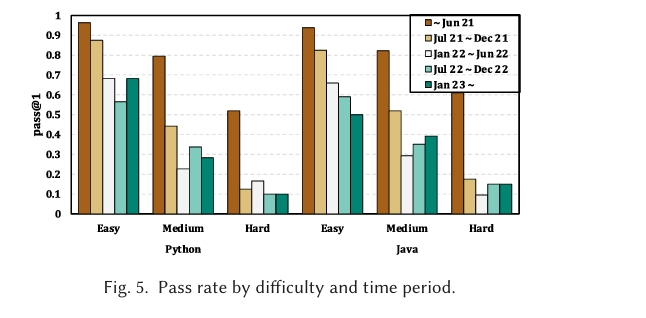
\includegraphics[width=10cm]{微信截图_20250208140421.jpg}

\begin{itemize}
\tightlist
\item
  程序越难，发现代码的质量问题越多
\end{itemize}

%\href{文件:微信截图_20250208140529.jpg}{600px\textbar{}无}

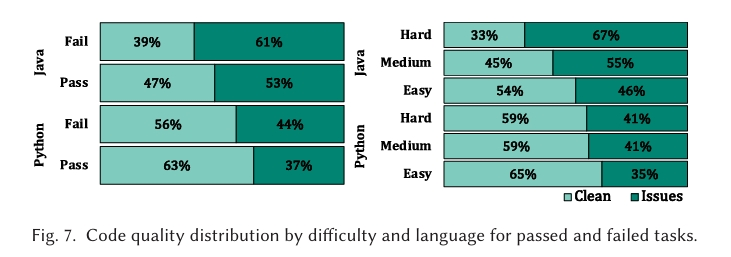
\includegraphics[width=10cm]{微信截图_20250208140529.jpg}

\begin{itemize}
\tightlist
\item
  下表是编译错误、输出结果有误、代码异味与维护性、性能等问题(issues)按语言、难度的分布：

  \begin{itemize}
  \tightlist
  \item
    代码异味例子：定义了变量，但没有使用
  \end{itemize}
\end{itemize}

表3： 按难度级别和编程语言的问题分布\\

%Screenshotfrom2025-02-1720-47-07.png


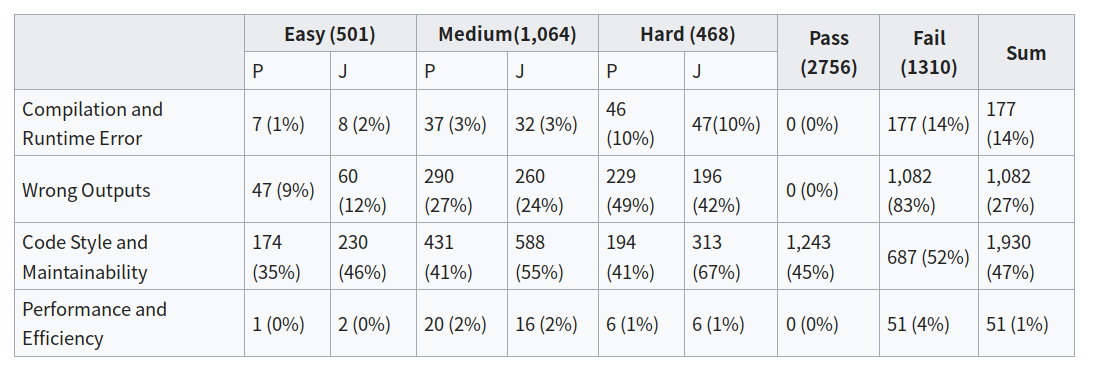
\includegraphics[width=10cm]{Screenshotfrom2025-02-1720-47-07.png}

%\textbar{}\}

\begin{itemize}
\tightlist
\item
  利用chatGPT
  AI功能自动修复，成功率按程序语言、难易度和错误类型分布：（下图）
\item
  从20\%左右起，最高能达到60\%
\end{itemize}

%\href{文件:微信截图_20250208140612.jpg}{600px\textbar{}无}

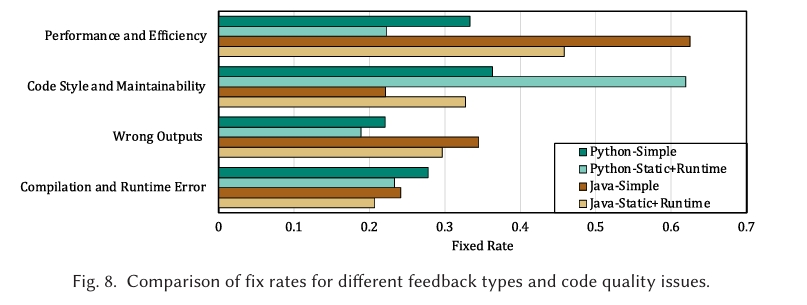
\includegraphics[width=10cm]{微信截图_20250208140612.jpg}

\hypertarget{ux53c2ux8003-references}{%
\subsection{参考 References}\label{ux53c2ux8003-references}}

\begin{enumerate}
\tightlist
\item
  E.L. Trist and K.W. Bamforth, 'Some Social and Psychological
  consequences of the Longwall method of Coal-Getting, Tavistock
  Institute (1951)
\item
  F.E. Emery and E.L. Trist, 'Socio-technical systems', in C.W.
  Churchman and M. Verhulst (eds.), ''Management Science, Models and
  Techniques, vol. 2, Pergamon (1960)
\item
  Ackoff,R.L. , J. Magidson and H.J. Addison, \emph{IDEALIZED DESIGN
  Creating an Organization's Future.} Wharton School Publishing (2006)
\item
  Barney, J.B. and Reeves M., 'AI won't give you a New Sustainable
  Advantage.' Harvard Business Review Sept-Oct, 2024.
\item
  Liu, Y. et al. 'Refining ChatGPT generated code: characterizing and
  mitigating code quality issues.' ACM Trans. Software Eng. Methodol.
  Vol.33, No.5, Art.116 June 2024.
\end{enumerate}


